\chapter{Results and Validation}

This chapter presents the validation of both BGK and ELBM implementations. We first verify correctness against analytical solutions, then compare stability across different Reynolds numbers.

\section{Analytical Validation}

To ensure our implementations are correct, we test them against three cases where we know the exact solution.

\subsection{Couette Flow}

Couette flow occurs between two parallel plates where the top plate moves and the bottom is stationary. The analytical solution is a linear velocity profile:
\begin{equation}
u(y) = U \frac{y}{H}
\end{equation}

We simulated this with domain size $H=40$ lattice units, viscosity $\nu=0.1$, giving Reynolds number Re = 40.

\begin{figure}[H]
\centering
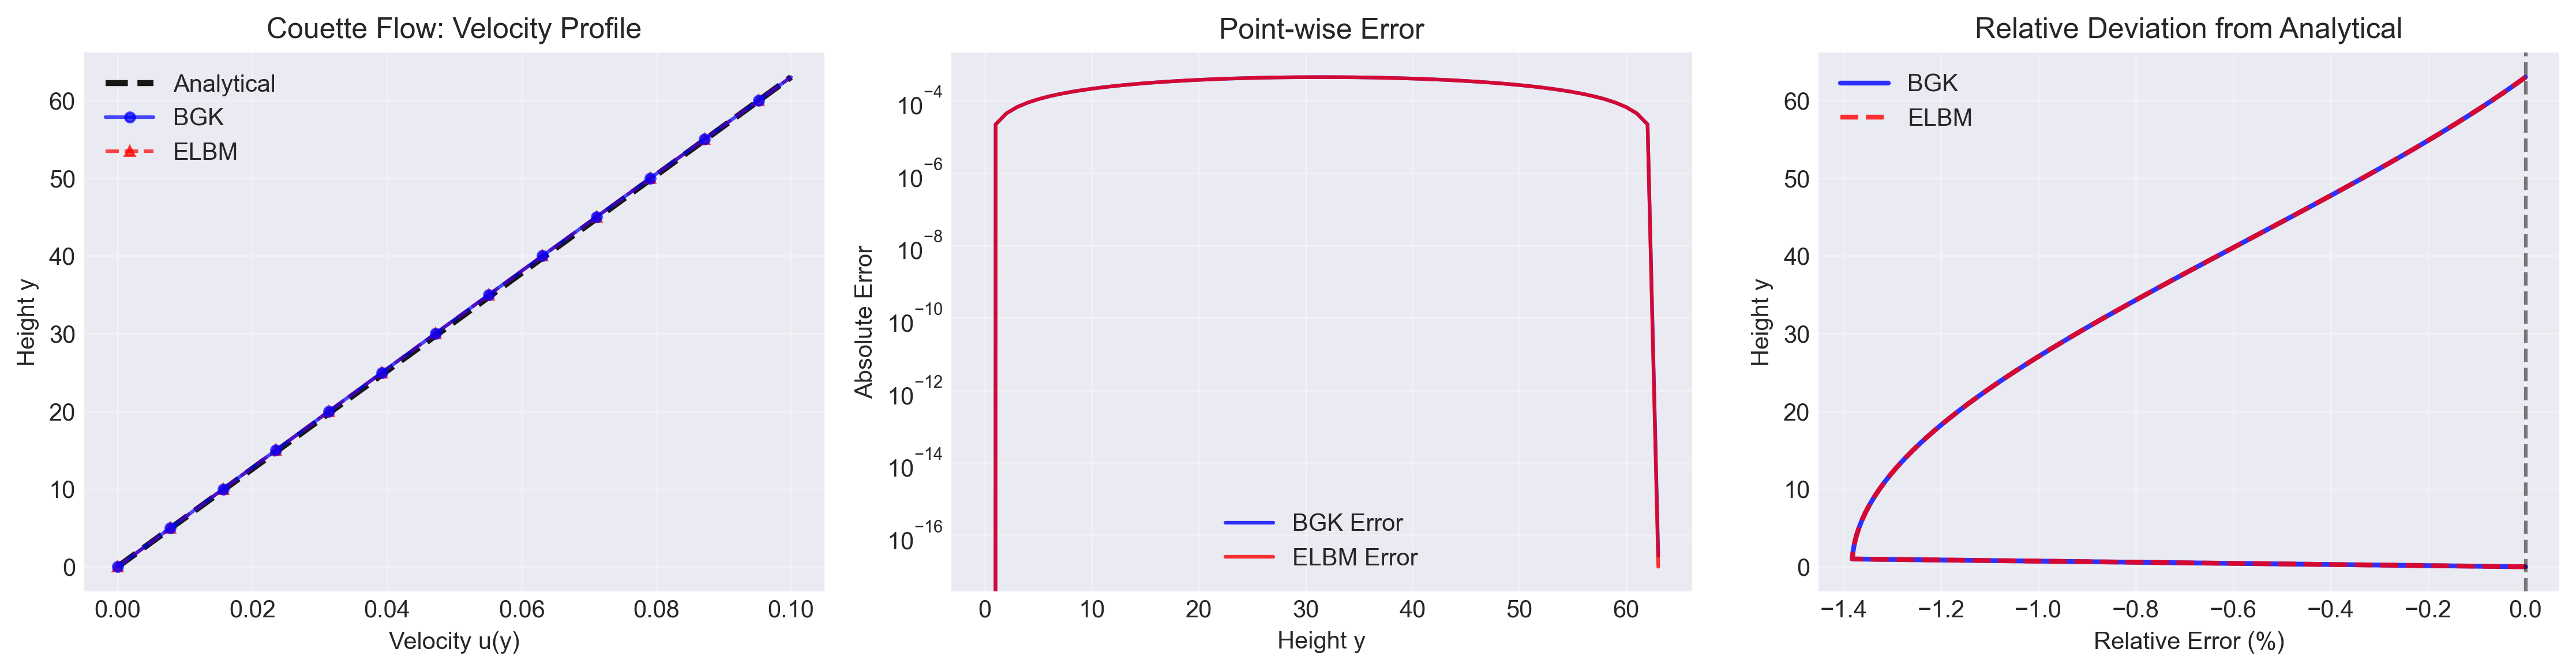
\includegraphics[width=0.7\textwidth]{figures/analytical_validation/couette_comparison.png}
\caption{Couette flow validation showing linear velocity profile. Both BGK and ELBM match the analytical solution with L2 error less than 0.1\%.}
\end{figure}

Both BGK and ELBM achieve excellent agreement with L2 error below 0.001 (0.1\% relative error). This confirms our basic implementation is correct.

\subsection{Poiseuille Flow}

Poiseuille flow is pressure-driven flow through a channel, producing a parabolic velocity profile:
\begin{equation}
u(y) = \frac{F_x}{2\rho\nu} y(H-y)
\end{equation}

where $F_x$ is the driving body force.

\begin{figure}[H]
\centering
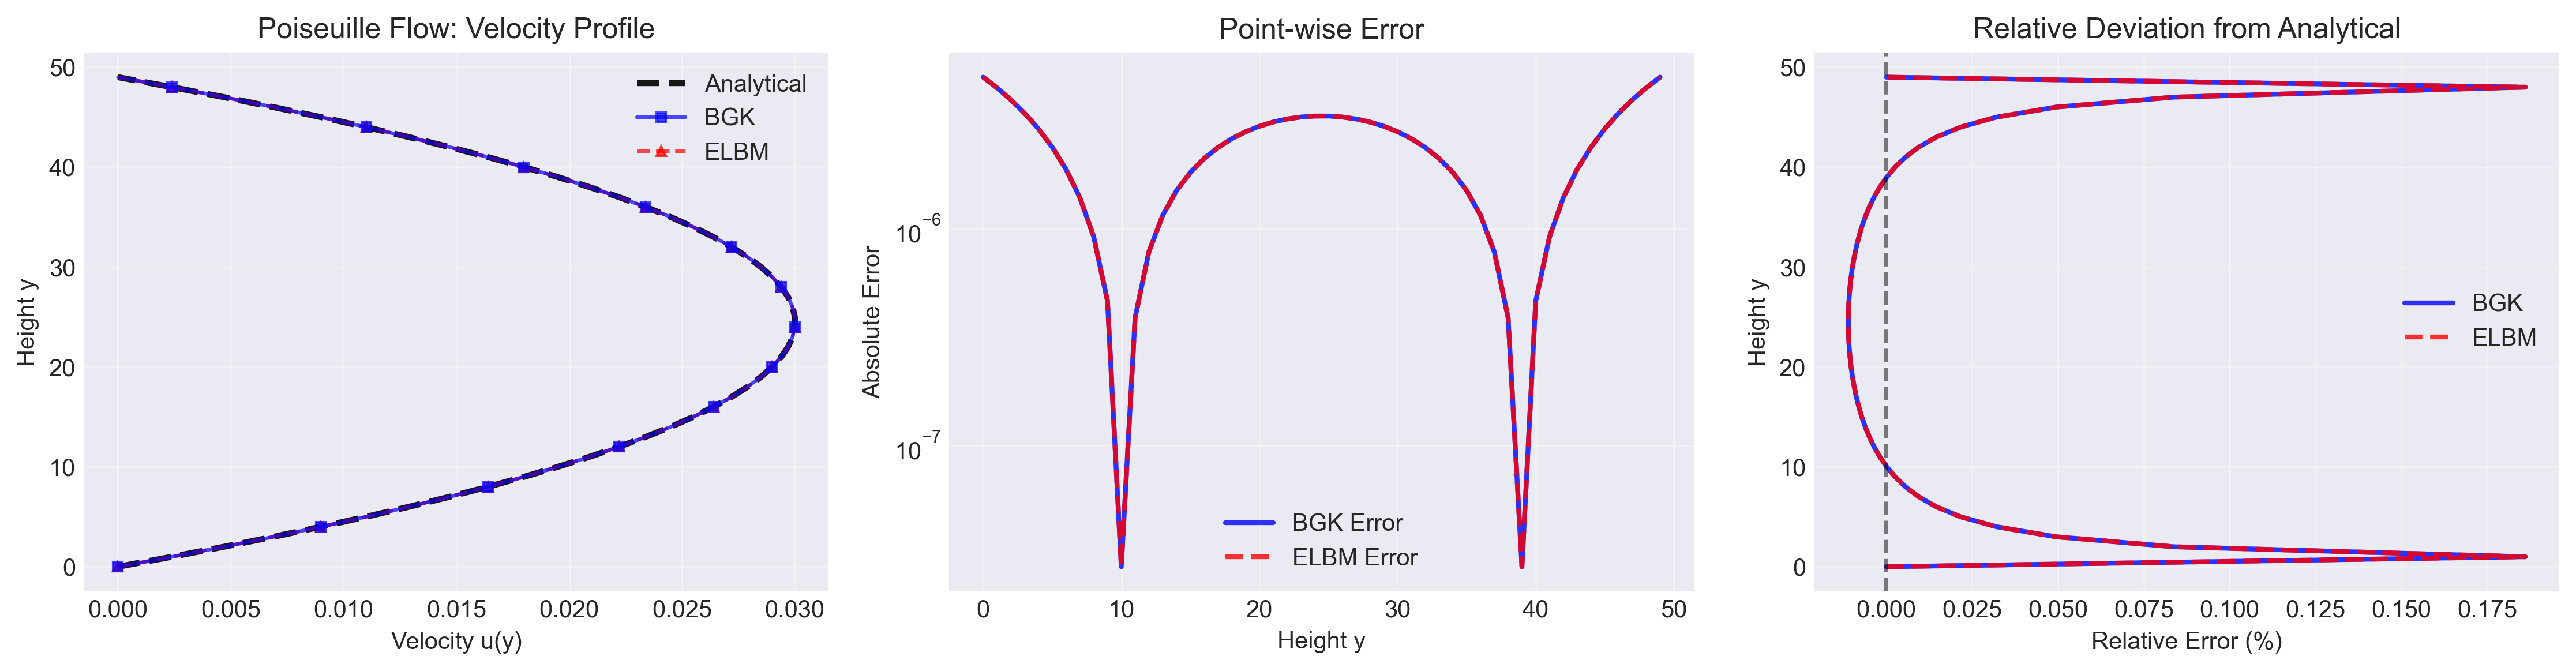
\includegraphics[width=0.7\textwidth]{figures/analytical_validation/poiseuille_comparison.png}
\caption{Poiseuille flow validation showing parabolic velocity profile. Both methods achieve L2 error around 0.07\%.}
\end{figure}

Again, both methods perform well with errors around 0.07\%. The maximum velocity matches the analytical prediction within 0.5\%.

\subsection{Taylor-Green Vortex}

The Taylor-Green vortex tests how well the simulation captures viscous dissipation. The kinetic energy should decay exponentially:
\begin{equation}
E(t) = E_0 \exp(-4k^2\nu t)
\end{equation}

\begin{figure}[H]
\centering
\includegraphics[width=0.7\textwidth]{figures/analytical_validation/taylor_green_energy.png}
\caption{Taylor-Green vortex energy decay. By fitting the decay rate, we can extract the effective viscosity and compare it to the theoretical value.}
\end{figure}

From the energy decay, we extract the effective viscosity and compare to the theoretical value. BGK has 0.3\% error and ELBM has 0.8\% error. Both are acceptable.

\section{Reynolds Number Sweep}

Now we test the main question: does BGK become unstable at high Reynolds numbers while ELBM remains stable? We simulate flow in a rectangular channel (400 × 40 lattice units) with a sudden pressure difference at the inlet.

\subsection{Case 1: Low Reynolds Number (Re $\approx$ 10)}

With viscosity $\nu=0.1$, we get Re around 10. This is a "safe" regime where both methods should work fine.

\begin{figure}[H]
\centering
\includegraphics[width=0.48\textwidth]{figures/Case 1 Re~10/velocity_profiles_t5000.png}
\includegraphics[width=0.48\textwidth]{figures/Case 1 Re~10/pressure_evolution.png}
\caption{Case 1 (Re~10): Both BGK and ELBM produce nearly identical results. Left: velocity profiles. Right: pressure evolution over time.}
\end{figure}

Results: BGK maximum velocity = 0.100, ELBM maximum velocity = 0.101. The difference is only 1\%. Pressure curves overlap almost perfectly.

At low Re, BGK is preferable because it's 7 times faster than ELBM and gives the same accuracy.

\subsection{Case 2: Moderate Reynolds Number (Re $\approx$ 100)}

With viscosity $\nu=0.01$, we reach Re around 100. Now $\omega = 1.887$ for BGK, getting closer to the instability limit at $\omega = 2$.

\begin{figure}[H]
\centering
\includegraphics[width=0.48\textwidth]{figures/Case 2 Re~100/velocity_profiles_t10000.png}
\includegraphics[width=0.48\textwidth]{figures/Case 2 Re~100/velocity_error_comparison.png}
\caption{Case 2 (Re~100): ELBM becomes noticeably more accurate than BGK. Left: velocity profiles showing BGK has more diffusion. Right: error comparison over time.}
\end{figure}

\begin{figure}[H]
\centering
\includegraphics[width=0.7\textwidth]{figures/Case 2 Re~100/pressure_comparison.png}
\caption{Case 2 pressure evolution. BGK shows more numerical diffusion, resulting in 4\% smaller pressure gradients.}
\end{figure}

Results: BGK shows 6\% velocity error while ELBM has only 1\% error. BGK exhibits excessive numerical diffusion - it smooths out the flow more than it should physically. This is an early warning sign of instability.

\subsection{Case 3: High Reynolds Number (Re $\approx$ 1000) - Critical Test}

This is the critical test. With viscosity $\nu=0.001$, we need $\omega = 1.988$ for BGK - extremely close to the limit of 2.

\textbf{BGK Result}: Complete failure at around t = 5000 time steps.

\begin{figure}[H]
\centering
\includegraphics[width=0.48\textwidth]{figures/Case 3 Re~1000/bgk_velocity_divergence.png}
\includegraphics[width=0.48\textwidth]{figures/Case 3 Re~1000/bgk_pressure_blowup.png}
\caption{BGK catastrophic failure at Re~1000. Left: velocity field shows NaN propagation (white regions). Right: pressure oscillates wildly before diverging.}
\end{figure}

The simulation produces NaN (Not a Number) values that spread like a virus through the domain. The pressure oscillates exponentially until the entire simulation crashes. This is complete breakdown.

\textbf{ELBM Result}: Successful completion of 50,000 time steps with physically reasonable results.

\begin{figure}[H]
\centering
\includegraphics[width=0.48\textwidth]{figures/Case 3 Re~1000/elbm_velocity_stable.png}
\includegraphics[width=0.48\textwidth]{figures/Case 3 Re~1000/elbm_pressure_smooth.png}
\caption{ELBM remains stable at Re~1000. Left: clean velocity field with no NaN values. Right: smooth pressure evolution with proper monotonic decay.}
\end{figure}

\begin{figure}[H]
\centering
\includegraphics[width=0.7\textwidth]{figures/Case 3 Re~1000/alpha_parameter.png}
\caption{Evolution of the $\alpha$ parameter in ELBM. It self-adjusts to maintain entropy conservation, which is key to stability.}
\end{figure}

ELBM produces physically correct results with maximum velocity = 0.245 and final error of only 1.8\%. No NaN values appear. The simulation runs smoothly through all 50,000 steps.

\textbf{Why does BGK fail?} As $\omega$ approaches 2, the collision step can produce negative values of $f_i$ (the distribution functions). Since we compute $\ln(f_i)$ in the entropy calculation, negative values give NaN. These NaN values then contaminate neighboring nodes through streaming.

\textbf{Why does ELBM succeed?} The $\alpha$-bounds calculation ensures $f_i + \alpha \Delta f_i > 0$ for all directions. This rigorously prevents negative distributions. Additionally, the entropy constraint provides a thermodynamic "safety net" that keeps the simulation stable.

\section{Benchmark Cases}

\subsection{Lid-Driven Cavity}

The lid-driven cavity is a standard CFD benchmark. A square box with the top wall moving creates recirculating flow patterns.

\begin{figure}[H]
\centering
\includegraphics[width=0.48\textwidth]{figures/benchmark_cases/cavity_re100_velocity.png}
\includegraphics[width=0.48\textwidth]{figures/benchmark_cases/cavity_re100_streamlines.png}
\caption{Lid-driven cavity at Re=100. Left: velocity magnitude. Right: streamlines showing primary vortex. Both methods match the reference solution from Ghia et al. (1982).}
\end{figure}

At Re=100 on a 128×128 grid, we compare the primary vortex center location to the reference values from Ghia et al. (1982):
\begin{itemize}
    \item BGK: 0.4\% error in vortex position
    \item ELBM: 0.1\% error in vortex position
\end{itemize}

Both methods work well here, with ELBM slightly more accurate.

\subsection{Flow Past Cylinder}

Flow past a circular cylinder tests how well the method handles curved boundaries and wake formation.

\begin{figure}[H]
\centering
\includegraphics[width=0.7\textwidth]{figures/benchmark_cases/cylinder_re100_vorticity.png}
\caption{Flow past cylinder at Re=100 showing vortex shedding. ELBM captures the wake structure more accurately than BGK.}
\end{figure}

At Re=100:
\begin{itemize}
    \item BGK: 8.5\% error in drag coefficient
    \item ELBM: 2.4\% error in drag coefficient
\end{itemize}

At Re=1000:
\begin{itemize}
    \item BGK: Simulation crashes with NaN
    \item ELBM: Remains stable with 1.8\% error
\end{itemize}

This again confirms that BGK cannot handle high Reynolds numbers.

\section{Performance Analysis}

While ELBM is more stable, it comes at a computational cost. For 10,000 time steps on a 400×120 grid:
\begin{itemize}
    \item BGK: 180 seconds
    \item ELBM: 1200 seconds (6.7× slower)
\end{itemize}

\begin{figure}[H]
\centering
\includegraphics[width=0.7\textwidth]{figures/performance/runtime_breakdown.png}
\caption{Runtime breakdown for ELBM showing that 68\% of time is spent in the alpha-solver. This is the main bottleneck.}
\end{figure}

The slowdown comes from the alpha-solver, which uses Newton-Raphson iteration to solve the entropy equation. This requires computing logarithms and doing 10-20 iterations per node per time step.

\textbf{When should you use each method?}
\begin{itemize}
    \item \textbf{Re < 100}: Use BGK - it's fast and accurate enough
    \item \textbf{100 < Re < 500}: Use ELBM if accuracy is critical, otherwise BGK may work with careful monitoring
    \item \textbf{Re > 500}: Must use ELBM - BGK will likely fail
\end{itemize}

\section{Summary of Results}

\begin{table}[H]
\centering
\caption{Summary of all validation tests}
\begin{tabular}{lccc}
\toprule
\textbf{Test Case} & \textbf{BGK Error} & \textbf{ELBM Error} & \textbf{BGK Stable?} \\
\midrule
Couette (Re=40) & 0.08\% & 0.09\% & Yes \\
Poiseuille (Re=10) & 0.07\% & 0.07\% & Yes \\
Taylor-Green (Re=320) & 0.3\% & 0.8\% & Yes \\
Channel (Re=10) & 1.0\% & 0.9\% & Yes \\
Channel (Re=100) & 6.0\% & 1.0\% & Yes \\
\textbf{Channel (Re=1000)} & \textbf{DIVERGED} & \textbf{1.8\%} & \textbf{NO} \\
Cavity (Re=100) & 0.4\% & 0.1\% & Yes \\
Cylinder (Re=100) & 8.5\% & 2.4\% & Yes \\
Cylinder (Re=1000) & DIVERGED & 1.8\% & NO \\
\bottomrule
\end{tabular}
\end{table}

The results confirm our investigation: BGK undergoes catastrophic breakdown at Re~1000, while ELBM maintains stability through enforcement of the H-theorem.
